\documentclass[./main.tex]{subfiles}
\graphicspath{{\subfix{./Abbildungen/}}}
\begin{document}
\renewcommand{\tasktitle}{Titel}
\renewcommand{\taskpoints}{3.5} %Gesamtpunktzahl der Aufgabe
\renewcommand{\taskweight}{8.7}
\aufgabenanfang % Beginn der Aufgabe


Dies ist ein Template zur Erstellung und Formatierung von IChO-Aufgaben (Klausurrunden 2–4) in \LaTeX. Am Ende des Dokuments sind einige weitere Hinweise zur Aufgabenerstellung gesammelt. 
Dies ist ein Beispiel für einen Einleitungstext zu einer Aufgabe. Es gibt zudem die Option diesen Text in einen Kasten zu setzen wie es ja bei der internationalen Runde üblich ist.  

\teilaufgabe{In diesem Bereich steht eine Teilaufgabe}{Hier kann ein Hinweis hinzugefügt werden}
\kasten{2.5cm}{
    Hiermit lässt sich ein Kasten erstellen zur Bearbeitung der Aufgabe.
    Die Länge des Kastens wird im Ersten Argument angegeben.
    Lösungskästchen folgen jeweils direkt auf die Aufgabenstellung – es gibt seit einigen Jahren keine Antwortbögen mehr!
    Musterlösung bzw Bewertungshinweise werden mit dem Command \textbackslash kommentar \{Hier direkt notiert\}:\\ %Zeilenumbruch
    \kommentar{Dies ist eine Musterlösung}\punkte{1}
}{Nur dieser Text erscheint im Endeeffekt in der Sch\"u lerversion}

Die folgenden Abschnitte enthalten einige Beispiel-Teilaufgaben. Die Aufgabenteile b) und c) dienen als Beispiele für Multiple-Choice-Aufgaben. 
\teilaufgabe{\operator{Kreuze an} welche Antwortm\"oglichekeiten hier richtig sind.}{Die Reihenfolge der richtigen Antworten wir in dem \textbackslash MC Command im 6.ten Argument mit einer Zeichenkette bspw.: oxoox, ausgedrückt die für die richtigen Antworten je ein x notiert}
Vor dem MC command folgt mit \textbackslash punkte wieder die Punktzahl \punkte{2}\\
\MC{A}{B}{C}{D}{E}{oxoox}

\teilaufgabe{\operator{Kreuze an} welche Antwortm\"oglichekeiten hier richtig sind.}{}
\MCvAnfang
\MCv{x}{Eine richtige Lösung}
\MCv{o}{Eine falsche Lösung}
\MCvEnde

In der folgenden Teilaufgabe folgt das Einfügen von OC Formeln bildern und OC Kästchen
\teilaufgabe
% \begin{figure}[H]
% \centering
% 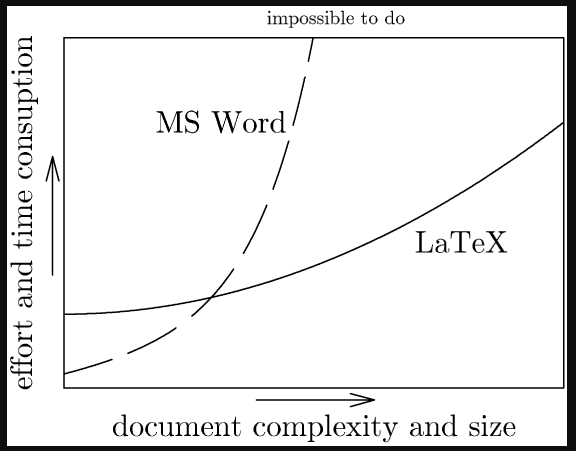
\includegraphics[width=0.7\textwidth]{test.png}
% \caption{Dies ist schlicht wahr }
% \label{A:test-Abb}
% \end{figure}
In Abbildung \ref{A:test-Abb} ist das und das dargestellt \ldots 
OC Sachverhalte können in zwei Formen eingefügt werden. Zum einen in der Latex eigenen Grafikvariante mit \textbackslash chemfig
\begin{scheme}[H]
    \centering
        \schemestart[0, 1, thick]
            \chemfig{
                        % 1
                =^[:210]% 2
                 -[:270]% 3
                =^[:330]% 4
                  -[:30]% 5
                  ~[:90,,,,lmb]% 6
                 -[:150]% 1
            }
            \+{1.5em, 1.5em, -0.508cm}
            \chemfig{
                       % 1
               =_[:330]% 2
                -[:270]% 3
               =_[:210]% 4
            }
            \arrow{->}
            \chemfig{
                        % 1
                  -[:30]% 2
                 =^[:90]% 3
                           (
                     -[:150]% 4
                    =^[:210]% 5
                     -[:270]% 6
                    =^[:330]% -> 1
                           )
                  -[:30]% 7
                 -[:330]% 9
                =_[:270]% 10
                 -[:210]% 8
                           (
                     -[:150]% -> 2
                           )
            }
        \schemestop
    \caption{Ich bin eine Diels-Alder-Reaktion.}
    \label{sc:da_reaction}
\end{scheme}
Zum anderen lässt sich aus ChemDraw eine .eps Datei exportiern und hier wie ein Bild Einfügen
\begin{scheme}[H]
    \centering
    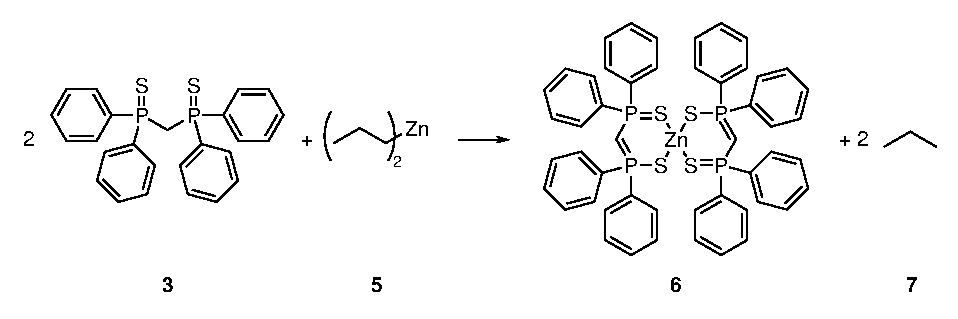
\includegraphics{Komplex.eps}
    \caption{Eine Synthese f\"ur die Tonne}
    \label{ACFKomplex}
\end{scheme}
Zu der Darstellung der OC- Lösungskästchen dient der Befehl: ---- \todo{Hier noch OC-Kasten nutzung einfügen}\\
(Unbekannte) Verbindungen werden mit römischen Zahlen bezeichnet. 
Eine Bezeichnung mit Buchstaben soll aufgrund möglicher Verwechslungen mit Elementsymbolen vermieden werden. 
Im Text werden die so nummerierten Moleküle (z. B. Verbindung 7) mit \textbackslash textbf hervorgehoben werden.\\
OC K\"asten werden mit dem Befehl \textbackslash kastenarray erstellt:\\
% \kastenarray
%     [] % Breite (kann weggelassen werden, dann an Inhalt angepasst)
%     {4cm} % Höhe
%     [0cm] % Abstand zwischen den Kästchen (kann weggelassen werden, dann 0cm)
%     [f] %t oder f: t - kein Abstand unter Kasten; f - Abstand unter Kasten (Optional; wenn weggelassen dann =t)
%     {Q,W} % Bezeichnungen
%     {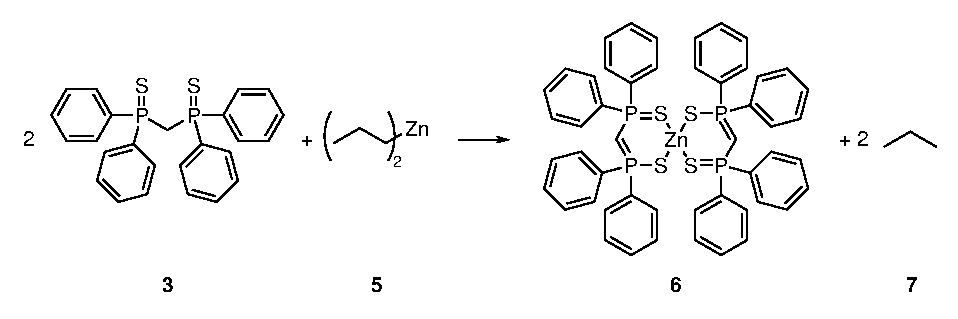
\includegraphics[width=5.5cm]{Komplex.eps},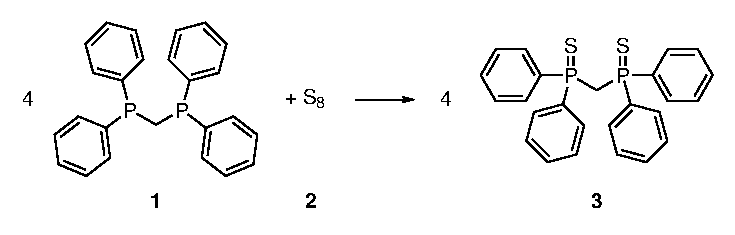
\includegraphics[width=5.5cm]{Ligand.eps}}% Inhalte mit Kommata seperieren
Man kann diese auch aneinander Reihen:
Noch zwei Kastenarrays.
% \kastenarray[7cm]{7cm}{1,2}{Molekuel1,Molekuel2}

% \kastenarray[7cm]{7cm}[0cm][]{3,4}{Molekuel3,Molekuel4}
\begin{align}
    pV &= nRT \label{G:test-Gl}\\
    a &= b
\end{align}
\textit{Hier soll kursiver Text stehen}.
In Gleichung \ref{G:test-Gl} ist das ideale Gasgesetz gezeigt \ldots 
Im Text sollten Vorzeichen wie bei $\delta-$/$\delta+$ besser au\ss{}erhalb des Mathemodusses stehen, aber ein richtiges Minuszeichen verwenden: $\delta$+/$\delta$\textminus{}

Hier kommt mal eine andere Aufz\"ahlung
\begin{enumerate}[(i)]
    \item Hallo
    \item Tsch\"uss
\end{enumerate}
Und danach wieder eine Teilaufgabe.
\teilaufgabe{\operator{Unterscheide} die verschiedenen Aufz\"ahlungen.}{}

\aufgabenende
\end{document}
